\documentclass[a4paper,oneside,12pt]{article}

\usepackage[american]{babel}

\usepackage{graphicx}
\usepackage{listings}

% figure counter???
%\usepackage{chngcntr}
%\counterwithout{figure}{chapter}
%\counterwithout{figure}{section}

%\setcounter{figure}{0}
%\renewcommand{\thefigure}{\arabic{section}.\arabic{figure}}

\newcommand{\half}{\frac{1}{2}}
\newcommand{\dt}{\Delta t}

% better tables
\usepackage{multirow}
\usepackage{booktabs}

% links
%\usepackage{color}
\usepackage[]{hyperref}
%bibliography
\usepackage[backend=biber,
style=numeric,
sorting=none,
natbib=true,
babel=other,
bibencoding=auto,
language=autobib,
giveninits=true]{biblatex}
% figures and tables
% \usepackage{caption}
% \captionsetup[figure]{labelfont=it,textfont=it}
% \captionsetup[table]{labelfont=it,textfont=it}
% \usepackage{subfig}

%%\usepackage[strict]{changepage}
% Define margins
%%\usepackage[left=2.5cm,right=2.5cm,top=2.5cm,bottom=2.5cm,includehead,includefoot,headheight=16pt]{geometry}

% Page headers
\usepackage{fancyhdr}
\fancyhf{}
\renewcommand{\headrulewidth}{0pt} 
\fancyhead[L]{\nouppercase{\leftmark}}
\cfoot{\thepage}
\pagestyle{fancy}


% Line spacing
%\usepackage{setspace}
%\setstretch{1.5}

% Defines uth-specific title page
%\usepackage{mieUTHtitle-en}
\usepackage{pgfplots} 
\usepackage{algorithm}
\usepackage{algpseudocode}

%Correct spelling of words. If the spelling of a word is incorrect and LaTex puts a hyphen at the wrong place on a line break then we give the correct spelling here.
%\babelhyphenation[greek]{Anti-here}
%-------------------------------------------

\begin{document}

% Fill in your details
\author{Alexander Pletzer, Chris Scott, Inna Senina, Lucas Bonnin and Romain Forestier}
\title{Implementation of cohort parallelisation in the Seapodym code}

\maketitle

%\frontmatter

\pagestyle{plain}

This report describes NeSI/REANNZ's consultancy project entitled ``SEAPODYM cohort parallelisation'' whose work was performed from May to September 2025.

\section{Statement of the problem}

SEAPODYM is a quantitative spatio-temporal model
of population dynamics that solves partial differential
equations with initial and boundary conditions in C++. 
The model is parameterized using a maximum
likelihood estimation approach that integrates georeferenced 
datasets obtained from industrial fishing and scientific campaigns.

The objective of this work is to parallelise the SEAPODYM code over cohorts. 
A cohort is a group of fish that are born at the same time. Each cohort 
can be integrated forward in time independently of other cohorts, until the cohort reaches a certain age and dies. 
At the next time step, a new cohort is born and integrated forward in time until it dies. Except 
at the first time step, the initial conditions of each cohort, however, depends on 
the density of the other cohorts at the previous time step. Thus, the integration of 
each cohort must take into account the state of the other cohorts and this requires 
careful consideration when parallelising the code.

An example of cohort time integration is shown below:
\begin{equation} \label{eq:cohorts}
\begin{array}{ccc}
0 & 1 & 2 \\
3 & 1 & 2 \\
3 & 4 & 2 \\
3 & 4 & 5 \\
6 & 4 & 6 \\
6 & 7 & 6
\end{array}
\end{equation}
Here, the vertical axis represents time increasing from top to bottom ($N_t = 6$). The horizontal axis represents the 
tasks than can be performed concurrently. Each row represents different age groups ($N_a = 3$). 
Moreover, each cohort is identified by an integer ($0, 1, \cdots 7$). 

Cohort 1 is one unit time older than cohort 2. Therefore cohort 1 dies one time step before cohort 2. Likewise,
cohort 0 is one time step older than cohort 1 and thus dies after the first time step. The number of time steps 
a cohort is integrated is $i = i_{beg} \cdots i_{end} - 1$ where $i_{beg} \geq 0$  and $i_{end} <= N_a$. Going back 
to our example, we have
\begin{table}[htbp]
    \centering % Centers the table horizontally
    \caption{Start and end integration indices for each cohort}
    \label{tab:cohort_indices}
    \begin{tabular}{c|cc} % Three centered columns
        \toprule % Top rule (from booktabs)
        cohort Id & $i_{beg}$ & $i_{end}$ \\
        \midrule % Middle rule (from booktabs)
        0 & 2 & 3 \\
        1 & 1 & 3 \\
        2 & 0 & 3 \\
        3 & 0 & 3 \\
        4 & 0 & 3 \\
        5 & 0 & 3 \\
        6 & 0 & 2 \\
        7 & 0 & 1 \\
        \bottomrule % Bottom rule (from booktabs)
    \end{tabular}
\end{table}
When a cohort dies, it is replaced by a new cohort at the next time step. To instantiate the new cohort, data will need 
to be transferred from the cohorts at the previous time step. Figure \ref{fig:cohort_deps} shows the dependency of the new cohorts on the older 
cohorts at different steps.
\begin{figure}[htbp]
    \centering
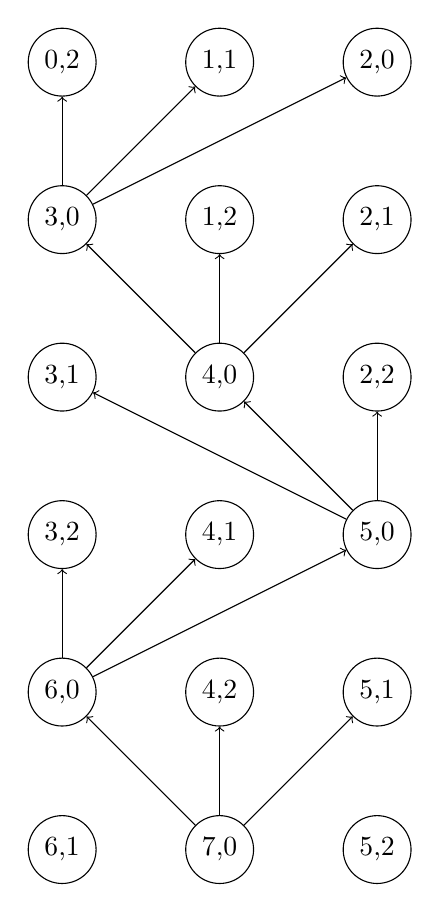
\begin{tikzpicture}[main/.style = {draw, circle}, node distance=2cm]
    \node[main] (02) {0,2};
    \node[main] (11) [right of= 02]{1,1};
    \node[main] (20) [right of= 11]{2,0};

    \node[main] (30) [below of= 02]{3,0};
    \node[main] (12) [right of= 30]{1,2};
    \node[main] (21) [right of= 12]{2,1};

    \node[main] (31) [below of= 30]{3,1};
    \node[main] (40) [right of= 31]{4,0};
    \node[main] (22) [right of= 40]{2,2};

    \node[main] (32) [below of= 31]{3,2};
    \node[main] (41) [right of= 32]{4,1};
    \node[main] (50) [right of= 41]{5,0};

    \node[main] (60) [below of= 32]{6,0};
    \node[main] (42) [right of= 60]{4,2};
    \node[main] (51) [right of= 42]{5,1};

    \node[main] (61) [below of= 60]{6,1};
    \node[main] (70) [right of= 61]{7,0};
    \node[main] (52) [right of= 70]{5,2};



    \draw[->] (30) -- (02);
    \draw[->] (30) -- (11);
    \draw[->] (30) -- (20);

    \draw[->] (40) -- (30);
    \draw[->] (40) -- (12);
    \draw[->] (40) -- (21);

    \draw[->] (50) -- (31);
    \draw[->] (50) -- (40);
    \draw[->] (50) -- (22);

    \draw[->] (60) -- (32);
    \draw[->] (60) -- (41);
    \draw[->] (60) -- (50);

    \draw[->] (70) -- (60);
    \draw[->] (70) -- (42);
    \draw[->] (70) -- (51);

\end{tikzpicture}
\caption{Dependency of cohort tasks on other cohort, step tuples. The first digit is the cohort Id and the second the step. }
    \label{fig:cohort_deps}
\end{figure}


\section{Task farming with dependencies on other tasks' steps}

We opted for a task farming approach. This involves creating a pool of tasks that can be executed concurrently
and a manager that assigns the tasks to the workers. Each task consists of advancing a cohort for multiple time steps.

In a classical task farming implementation, the manager starts by assigning tasks to the workers. This involves sending a message to each worker, along with 
some input parameters. Each worker then executes the task and reports the results back to the manager, who then assigns a new task to the worker. 
When no more tasks are available, the manager sends a message to the workers to shut down. Task farming is particularly suitable when tasks take a different amount of time to execute, either because of the nature of the task or because of
of varying computational loads or because of task heterogeneity.

Clearly, the dependencies between tasks and sub-tasks shown in Fig. \ref{fig:cohort_deps} prevents us from using a naive task farming approach. In our case, tasks can only be started when 
other task steps have been completed. In other words, a task corresponding to advancing a cohort at a given step can only be started once all its prerequisite tasks 
(as indicated by the arrows in Fig. \ref{fig:cohort_deps}) have finished. This requires the manager to keep track of task dependencies and only dispatch tasks to workers when 
their dependencies are satisfied.

We start by describing a worker's task. A worker waits for a task to be assigned by the manager. A task has a identification number \verb|workerId| that fully describes the task to accomplish.
The worker reports back the status of the execution of each task to the manager. The corresponding pseudo-code is:

\begin{algorithm}
\caption{A worker's pseudo-code.}
    \begin{algorithmic}[1] % [1] for line numbering
    \While {true}

        taskid = \Call{getTaskIdFromManager}{};
        \If {taskid $< 0$}
            Break
        \EndIf

        \Comment{Perform the task, stepping from stepBeg to stepEnd - 1}   
        \State \Call{taskFunc}{taskid, stepBeg, stepEnd}

        \Comment{Notify the manager that this worker is available again}
        \State \Call{sendSignalToManager}{DONE}
    
    \EndWhile
\end{algorithmic}
\label{algo:worker}
\end{algorithm}

The task function defined in Algorithm \ref{algo:worker} is responsible for advancing the cohort associated with \verb|taskid| from \verb|stepBeg| to \verb|stepEnd - 1|:
\begin{algorithm}
\caption{The task function executed by the worker.}
    \begin{algorithmic}[1] % [1] for line numbering
\Function{MyFunction}{taskid, stepBeg, stepEnd}
    \State data = \Call{getDataFromManager}{taskid}
    \State cohort = \Call{createCohort}{taskid}
    \Comment{Advance a cohort}
    \For {step = stepBeg to stepEnd - 1}
        \State \Call{stepForward}{cohort}
        \State \Call{sendStepCompleteMessageToManager}{taskid, step}
    \EndFor
\EndFunction
\end{algorithmic}
\label{algo:worker}
\end{algorithm}



\section{Summary and future work}
   

\end{document}